%% NOTES:
%%    do we want to explore for larger S?  Does false positive rate change?

\documentclass[12pt]{article} \usepackage{simplemargins}
\usepackage[pdftex]{graphicx} \graphicspath{{figures/}}

\setlength{\parindent}{0pt} \setlength{\parskip}{1.6ex}
\setallmargins{1in} \linespread{1.6}

\begin{document}

\title{A probabilistic framework for compressible assembly graphs}
\author{Jason Pell, Arend Hintze, Rosangela Canino-Koning, C. Titus Brown}

\maketitle

\section{Abstract}

We introduce a fast and lightweight representation of DNA k-mer graphs
based on a probabilistic representation.  This graph has a one-sided
error that is precisely tunable and yields predictable degradation of
graph properties as memory usage is decreased. This degradation as the false 
positive rate of the data structure increases relates to percolation theory. Through 
simulation, we found that the percolation threshold for a k-mer graph 
is $\sim 0.183$. We show that this
graph representation can be used to characterize the structure of
large assembly graphs.

\section{Introduction}

Within the past decade, the volume of sequence data generated
from next-generation sequencing platforms such as Illumina and 454
has outpaced the computational resources needed for
analysis. Currently, the memory needs for sequencing projects 
are high. Recent sequencing efforts such as the human gut
microbiome\cite{pmid20203603}, cow rumen\cite{pmid21273488}, and the 
human genome\cite{pmid21187386} require large computers with 512GB of memory
or more to construct their assemblies.  
Sequencing companies continue to innovate in developing new 
methods to produce longer reads, fewer errors, 
and deeper coverage. However, this further contributes 
to the difficulty in computational 
analysis of the data, and better scaling data structures and algorithms 
must be developed. Today, high memory requirement for sequence assembly is
among the biggest bottlenecks that we face in efficiently analyzing
sequence data. To resolve this issue, we present a novel application
of the Bloom filter data structure\cite{bloom} for storing and traversing de
Bruijn graphs in memory, which reduces memory requirements for some 
operations related to DNA sequence assembly.

The goal of de novo assembly is to assemble individual disconnected
reads into a consensus sequence based on overlaps and mate-pair
information. Before the advent of next-gen platforms, Sanger
sequencing was the primary method used for sequencing. To assemble 
these datasets, the reads were checked for overlaps through an 
all-by-all comparison, and an overlap graph was created.
an all-by-all comparison by constructing a graph\cite{assemblyreview}.
Using the overlap graph, the assembler 
performs several multiple sequence alignments to find a consensus sequence. 
If paired-end information is available, some repetitive regions in the 
genome are resolved, and scaffolds between contigous sequences are 
created. This class of assemblers is generally called 
``Overlap-Layout-Consensus.'' Examples include
Arachne\cite{arachne}, Celera\cite{celera}, Newbler\cite{newbler}, and 
PCAP\cite{pcap}. However, with next-gen sequencing 
platforms such as 454 and Illumina, much larger datasets of shorter reads 
are generated. With the Illumina Hi-Seq 2000 platform, up to 200 
gigabases of sequence can be generated 
in around 7 days with reads in excess of 100 bp. The assembly of 
these reads requires different
algorithms and also a much larger amount of memory. Originally developed to 
handle repeat structures in Sanger datasets, a new approach using de Bruijn 
graphs (DBG) was developed\cite{pmid11504945}, which scales with the number 
of ``k-mers'' as opposed to reads.
In a de Bruijn
graph approach, reads are broken down along a sliding window into words of fixed
size $k$, or k-mers, and overlaps are implicitly represented as shared (k-1)-mers.
De Bruijn graph assemblers then try to find an Euler path through
this graph, which is then output as an assembled contig\cite{assemblyreview}.

As next-generation sequencing platforms became prominent, the DBG approach
became the preferred method for assembling these types of datasets
because an all-by-all comparison of reads is infeasible in situations where 
computational resources are limited and/or dataset sizes are massive. While DBG
approaches are generally more memory-efficient than OLC approaches,
they do not scale.  It
is clear that more efficient methods are needed to handle the
increasing size of sequence datasets. This need is
prevalent in the area of metagenomics, and is especially
needed for high diversity
microbial communities. Due to the high number of microbial species 
in environmental samples, it is generally difficult to obtain high coverage 
for low abundant species. This 
requires very deep coverage, which introduces novel k-mers from both 
errors and sequence that 
would be difficult to obtain with lower coverage. In a similar fashion, 
low-expressed genes in mRNAseq samples are difficult to detect without deep 
sequencing. Due to this need for high coverage in many sequencing 
domains, the memory scaling issue must be addressed.

Driven by the need to scale, we explore the use of a 
Bloom filter variant to create a compressible graph 
% @JAP expand on more Bloom filter/Bioinformatics-related stuff
representation. Bloom filters have been used for Bioinformatics applications 
in the past\cite{pmid20472541, haskell, pmid20426693}. We show that this method drastically
reduces memory requirements and that the drawbacks from using such a method 
with false positives are negligible. Furthermore, we show that our 
approach performs well under a specific false positive rate. We also 
briefly discuss techniques for using the probabilistic k-mer graph 
to study assembly graph structure and potentially improve assembly by 
graph decomposition, repeat filtering, and other approaches.

\section{Methods}

\subsection{Data Structure Implementation}
We use a variation of the Bloom filter data structure to store k-mers
in memory. Rather than using multiple hash functions with a single
hash table, we use a different hash table for each hash
function. Given a k-mer of interest, each table is queried for the
presence of a k-mer until the k-mer cannot be found in a hash
table. In order for a k-mer to be considered present in the dataset, 
the k-mer must be found in all of the hash tables. On the other hand, 
if a k-mer is not present in even one hash table, then it is certainly 
not in the dataset. As a result, there is a one-sided error where 
false positives are possible but false negatives are not.

\subsection{Calculating Data Structure Properties}
Many properties of Bloom filters such as the optimal number of hash functions 
and the false positive rate are simple to calculate. The properties 
of our Bloom filter variant, which 
uses a separate hash table for each hash function, is essentially the 
same as a classical Bloom filter. To calculate the false positive rate, we 
take the product of the occupancy of each hash table; that is,
\begin{displaymath}
P_f = \prod_{h \in H} occ(h)
\end{displaymath}
where $h$ is a hash table in the set of hash tables $H$, $occ$ denotes 
the occupancy (proportion of bits set) for a hash table, and $p_f$ is 
the false positive rate.

\subsection{Percolation Threhold Estimation}
To calculate the rate at which aberrant connectivity is generated, 
we randomly add k-mers to the data structure 
and continually calculate the false positive rate and size of the largest connected 
component. This allows us to sample the relative size of the largest component for every 
given $p$ (probability that a k-mer is present) as well as the cluster size distribution. 
At the percolation threshold this cluster size distribution must be scale-free(citation?). 
We then find at what value of $p$ the resulting 
distribution in logarithmic 
scale can be better fitted in a linear or quadratic fashion using 
the F-value
\newline
\newline
% @JAP I tried to make the equations look better, but I am also somewhat limited
% in my LaTeX knowledge on this 
\begin{displaymath}
F=\frac{\frac{RSS_1-RSS_2}{p_2-p_1}}{\frac{RSS_2}{n-p_2}}.
\end{displaymath}
Finally, to handle the finite size sampling error the data is binned using the 
threshold binning method\cite{adami2002critical}. The critical value for percolation is found 
by finding the local maxima.

\subsection{Software and Software Availability}

We have also developed a software package named khmer, which
implements our probabilistic de Bruijn graph.  It is written in C++
and Python 2.6 and is released under the BSD license. The graphviz software 
package was used for graph visualizations. The scripts to 
generate the figures of this paper along with khmer are freely available
at: https://github.com/ctb/khmer.

\section{Results}

\subsection{Using Bloom Filters To Store K-mers}
It is easy to show that the many
calculable properties such as optimal number of hash functions that
can be determined for Bloom filters apply to our variation as well.  
Another advantage to
using a Bloom filter is that a linear increase in the amount of memory
used creates an exponential improvement in the false positive
rate. For example, $\sim4.78$ bits per k-mer are needed for a false
positive rate of 10\% while $\sim6.22$ bits per k-mer are need for a false
% @JAP This doesn't show an exponential improvement since there are only two data points
positive rate of
5\%. As with other hash-style data structures, Bloom filters have a
fast lookup time, which is $O(h)$ when there are $h$ hash tables to query
for k-mer presence. 

\subsection{Using The Bloom Filter As A K-mer Graph}
Having stored the k-mers into a Bloom filter, we are able to traverse
the corresponding k-mer graph. We let each k-mer be a vertex, where
the reverse complement of a k-mer is considered the same
vertex. Furthermore, we treat the graph as a simple graph as opposed
to a multigraph or digraph, which means that there can be no
self-loops or parallel edges between vertices/k-mers. Each k-mer can
have up to eight neighbors, which are any of the other k-mers that
 share a $k-1$ 
overlap. Some k-mers can have less than adjacent k-mers: an alternating k-mer
(e.g. ATATA...) has seven neighbors and k-mers with each position
having the same base (e.g. AAAAA...) has six. Our graph representation is 
constant in its memory usage, so only ancillary information such as list of 
nodes visited or waypoints in the graph consume addition memory.
 
In contrast to an exact
approach, there is a chance that a k-mer will be adjacent to a k-mer
that does not actually exist in the original dataset due to the false
positive rate from the Bloom filter. If this probability is too high,
it can be impossible to traverse given high enough K. For example, if
K is set to 32, no modern computer can explore each k-mer in a
reasonable period of time. It is intuitively clear that when most real k-mers 
have at least one erroneous neighbor ($p_f \approx \frac{1}{8}$), false connections 
between real k-mers are likely to develop. However, it is not immediately clear 
at what false positive rate this occurs without simulation or an analytic 
solution.

%@JAP This part is stolen basically word for word from the grant proposal
This graph structure is effectively compressible because one can choose a larger 
or smaller size for the underlying Bloom filters; a larger size admits fewer 
node false positives, while a smaller size admits more. By relying on Bloom 
filters, the data structure is effectively constant memory: no extra memory is 
used as additional data is added. However, as memory is decreased or data 
is increased, only false positive nodes and edges are gained, so 
compressing the graph results in a more tightly interconnected graph.

\subsection{Effect Of False Positives on Local Graph Structure}
To see how erroneous neighbors created by false positives can alter 
the local graph structure, we randomly generated a 1,000bp sequence 
and added the first 31-mer to
the end to create a circular chromosome with 1,000 31-mers. Then,
using four different false positive rates ($p_f$=0.01, 0.05, 0.10, and
0.15), we explored the graph using breadth-first search beginning at
the first 31-mer. 
The graphs in Figure 
1 demonstrate how
the local graph structure begins to change while the original circular
graph remains intact with no erroneous paths between k-mers that are
truly present in the originally generated sequence. Because the k-mer
space is so large for high enough K, a relatively high false positive 
rate ($\sim$ 15\%) is still 
unlikely to connect components
together erroneously. We also note that when the false positive
rate is sufficiently high, the resulting graph would be
impossible to visualize for high values of $k$ (e.g. $\ge 25$). 

\begin{figure}
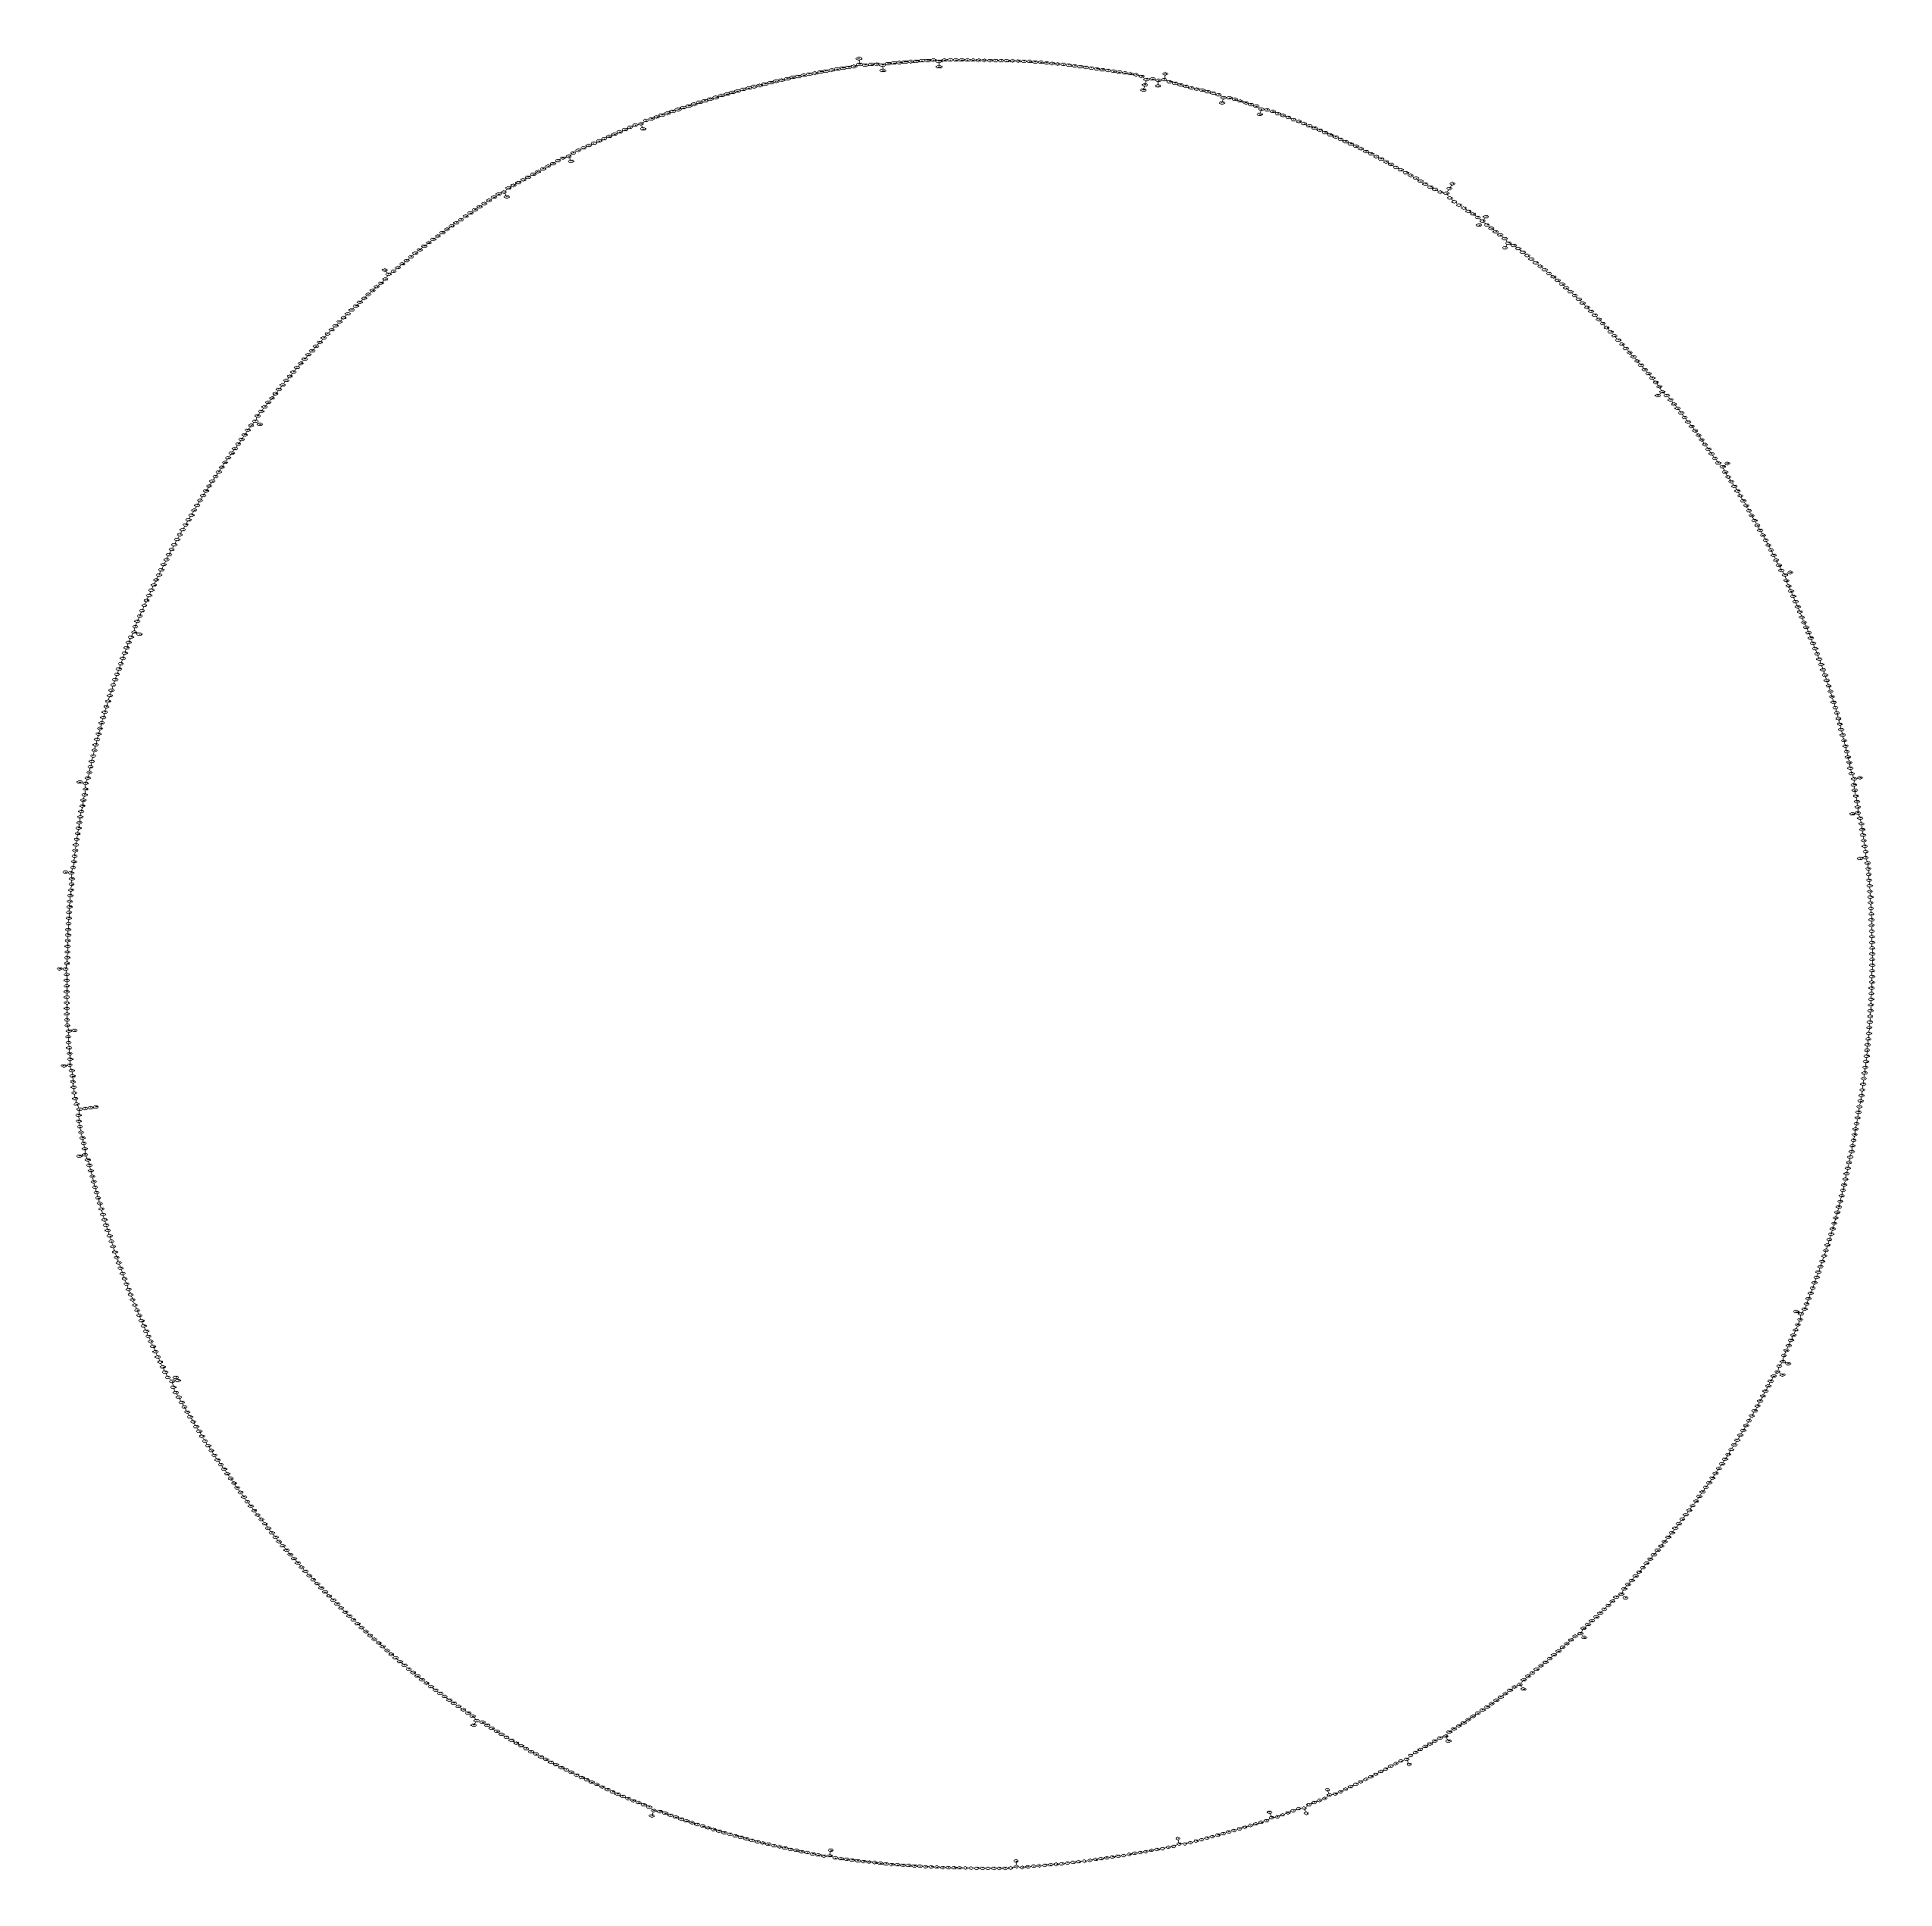
\includegraphics[width=3in]{figures/f3b001}
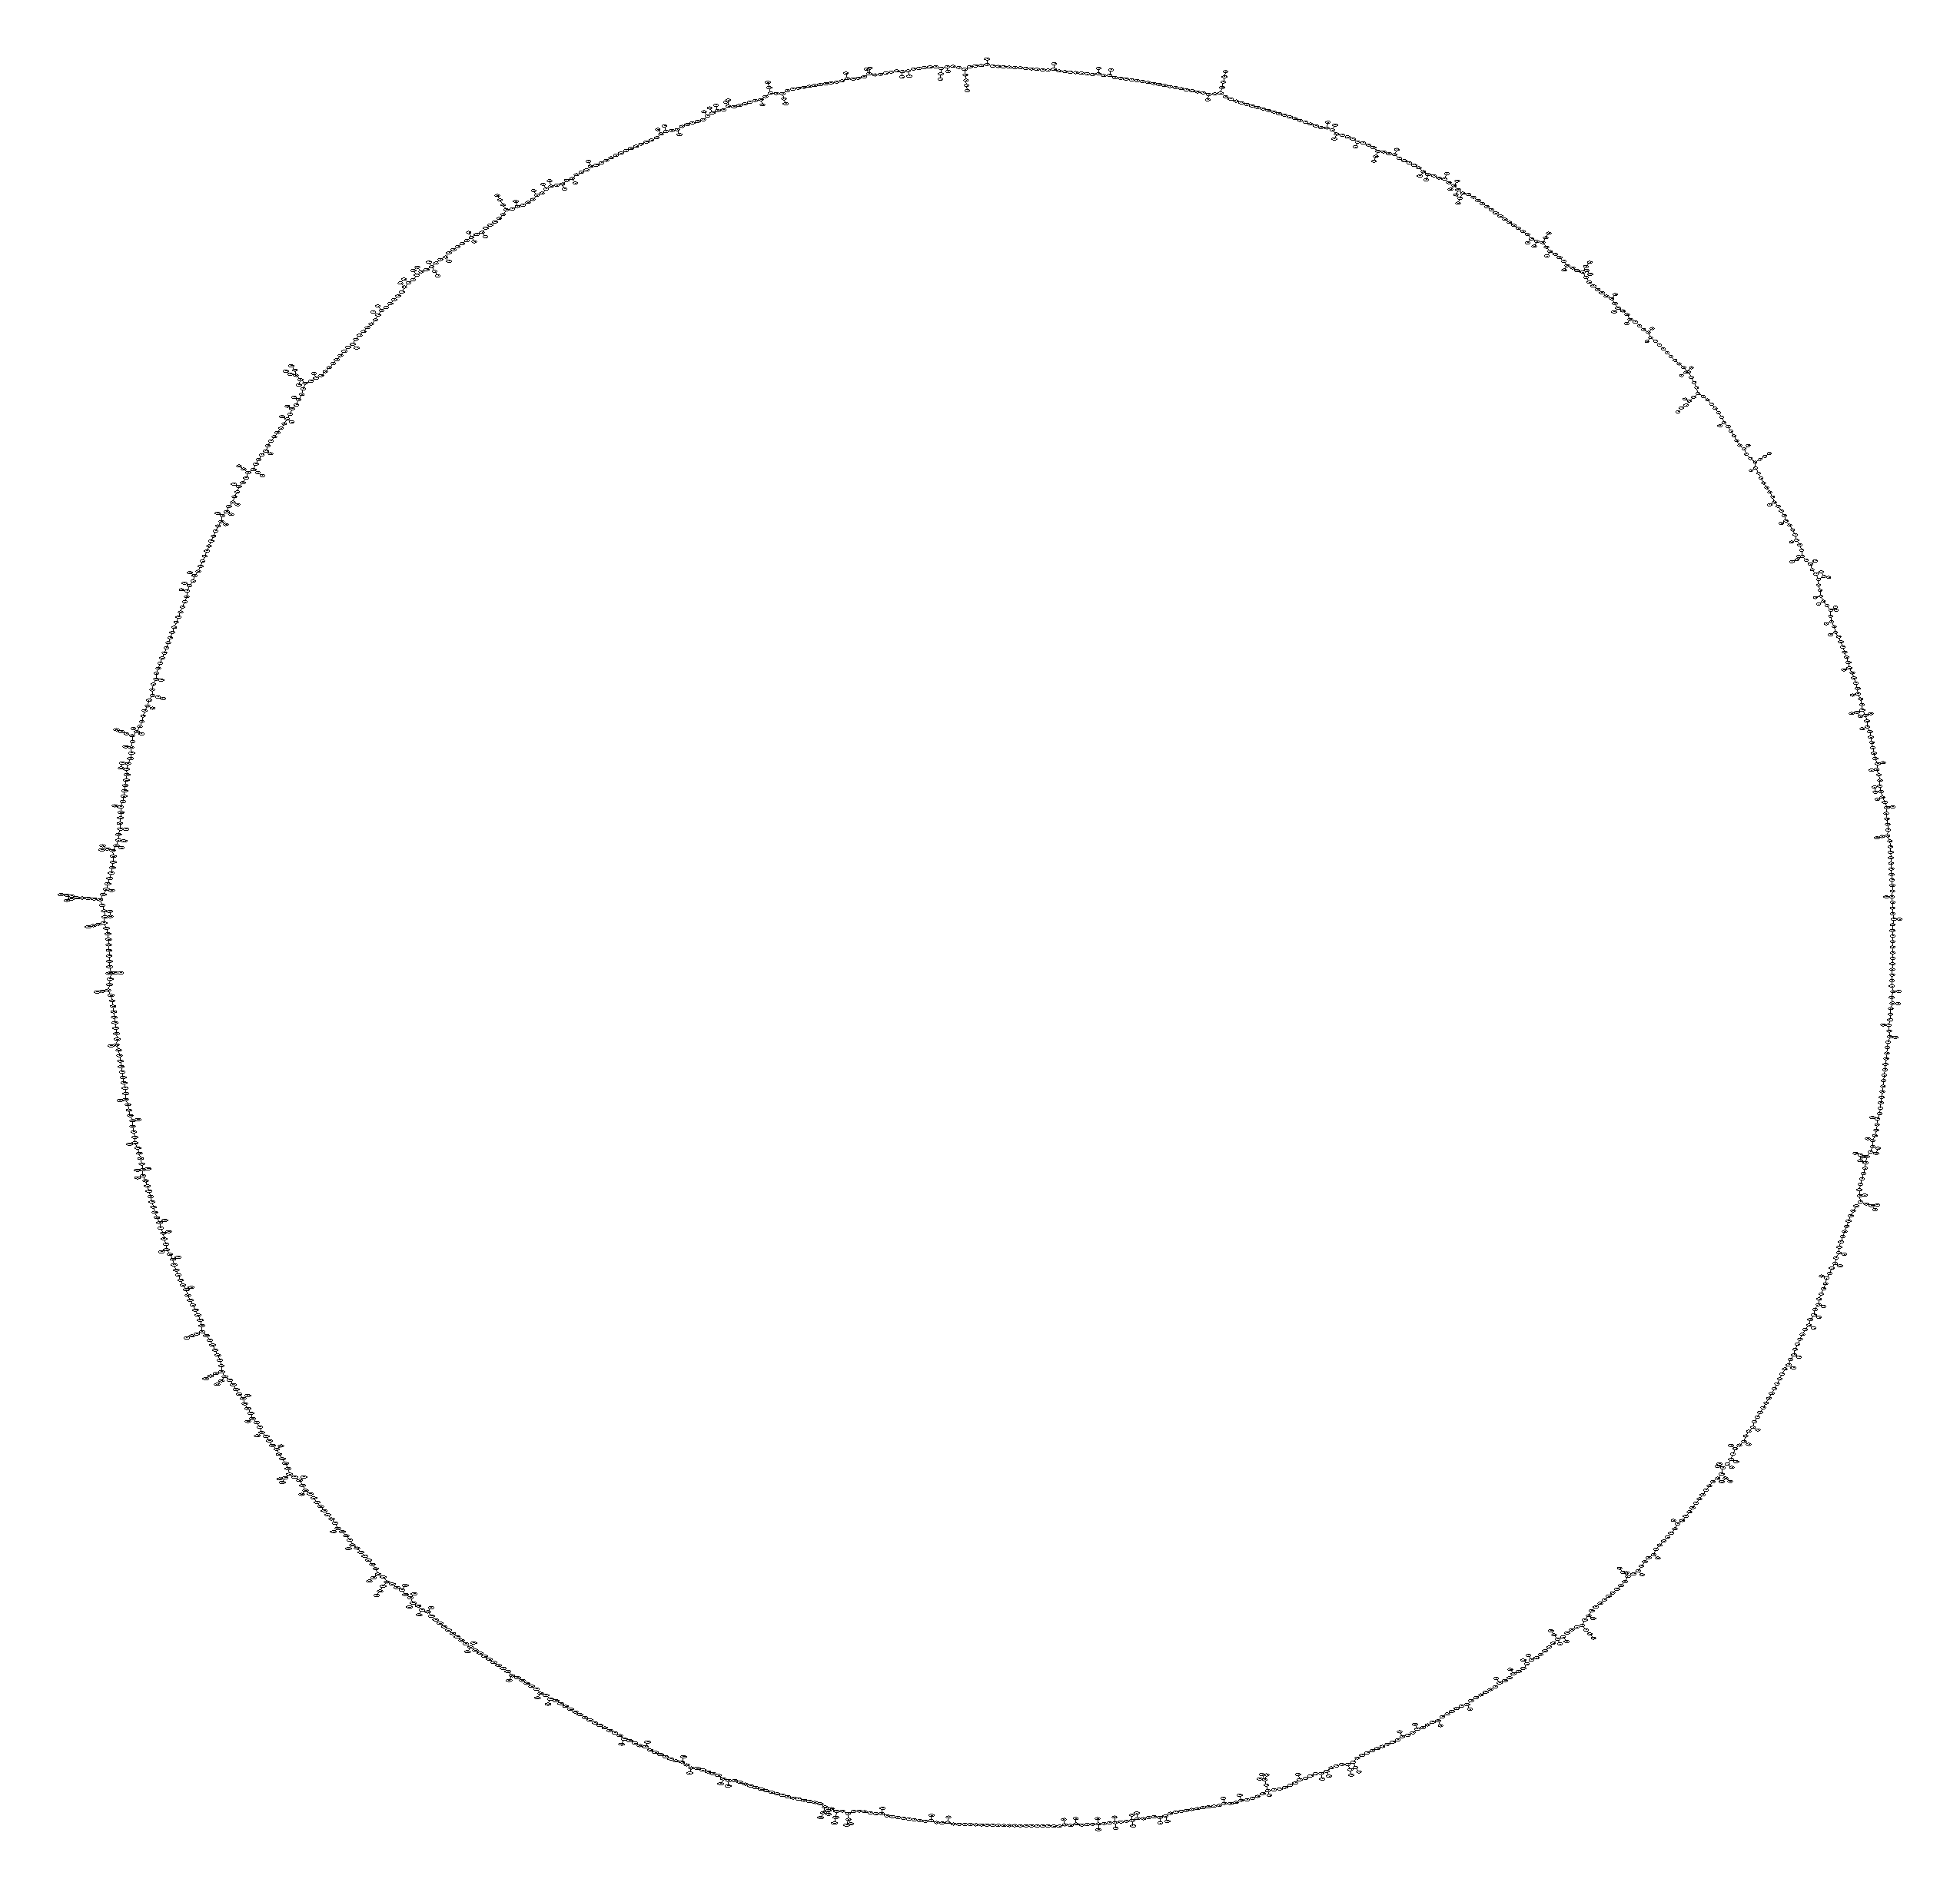
\includegraphics[width=3in]{figures/f3b005}\\
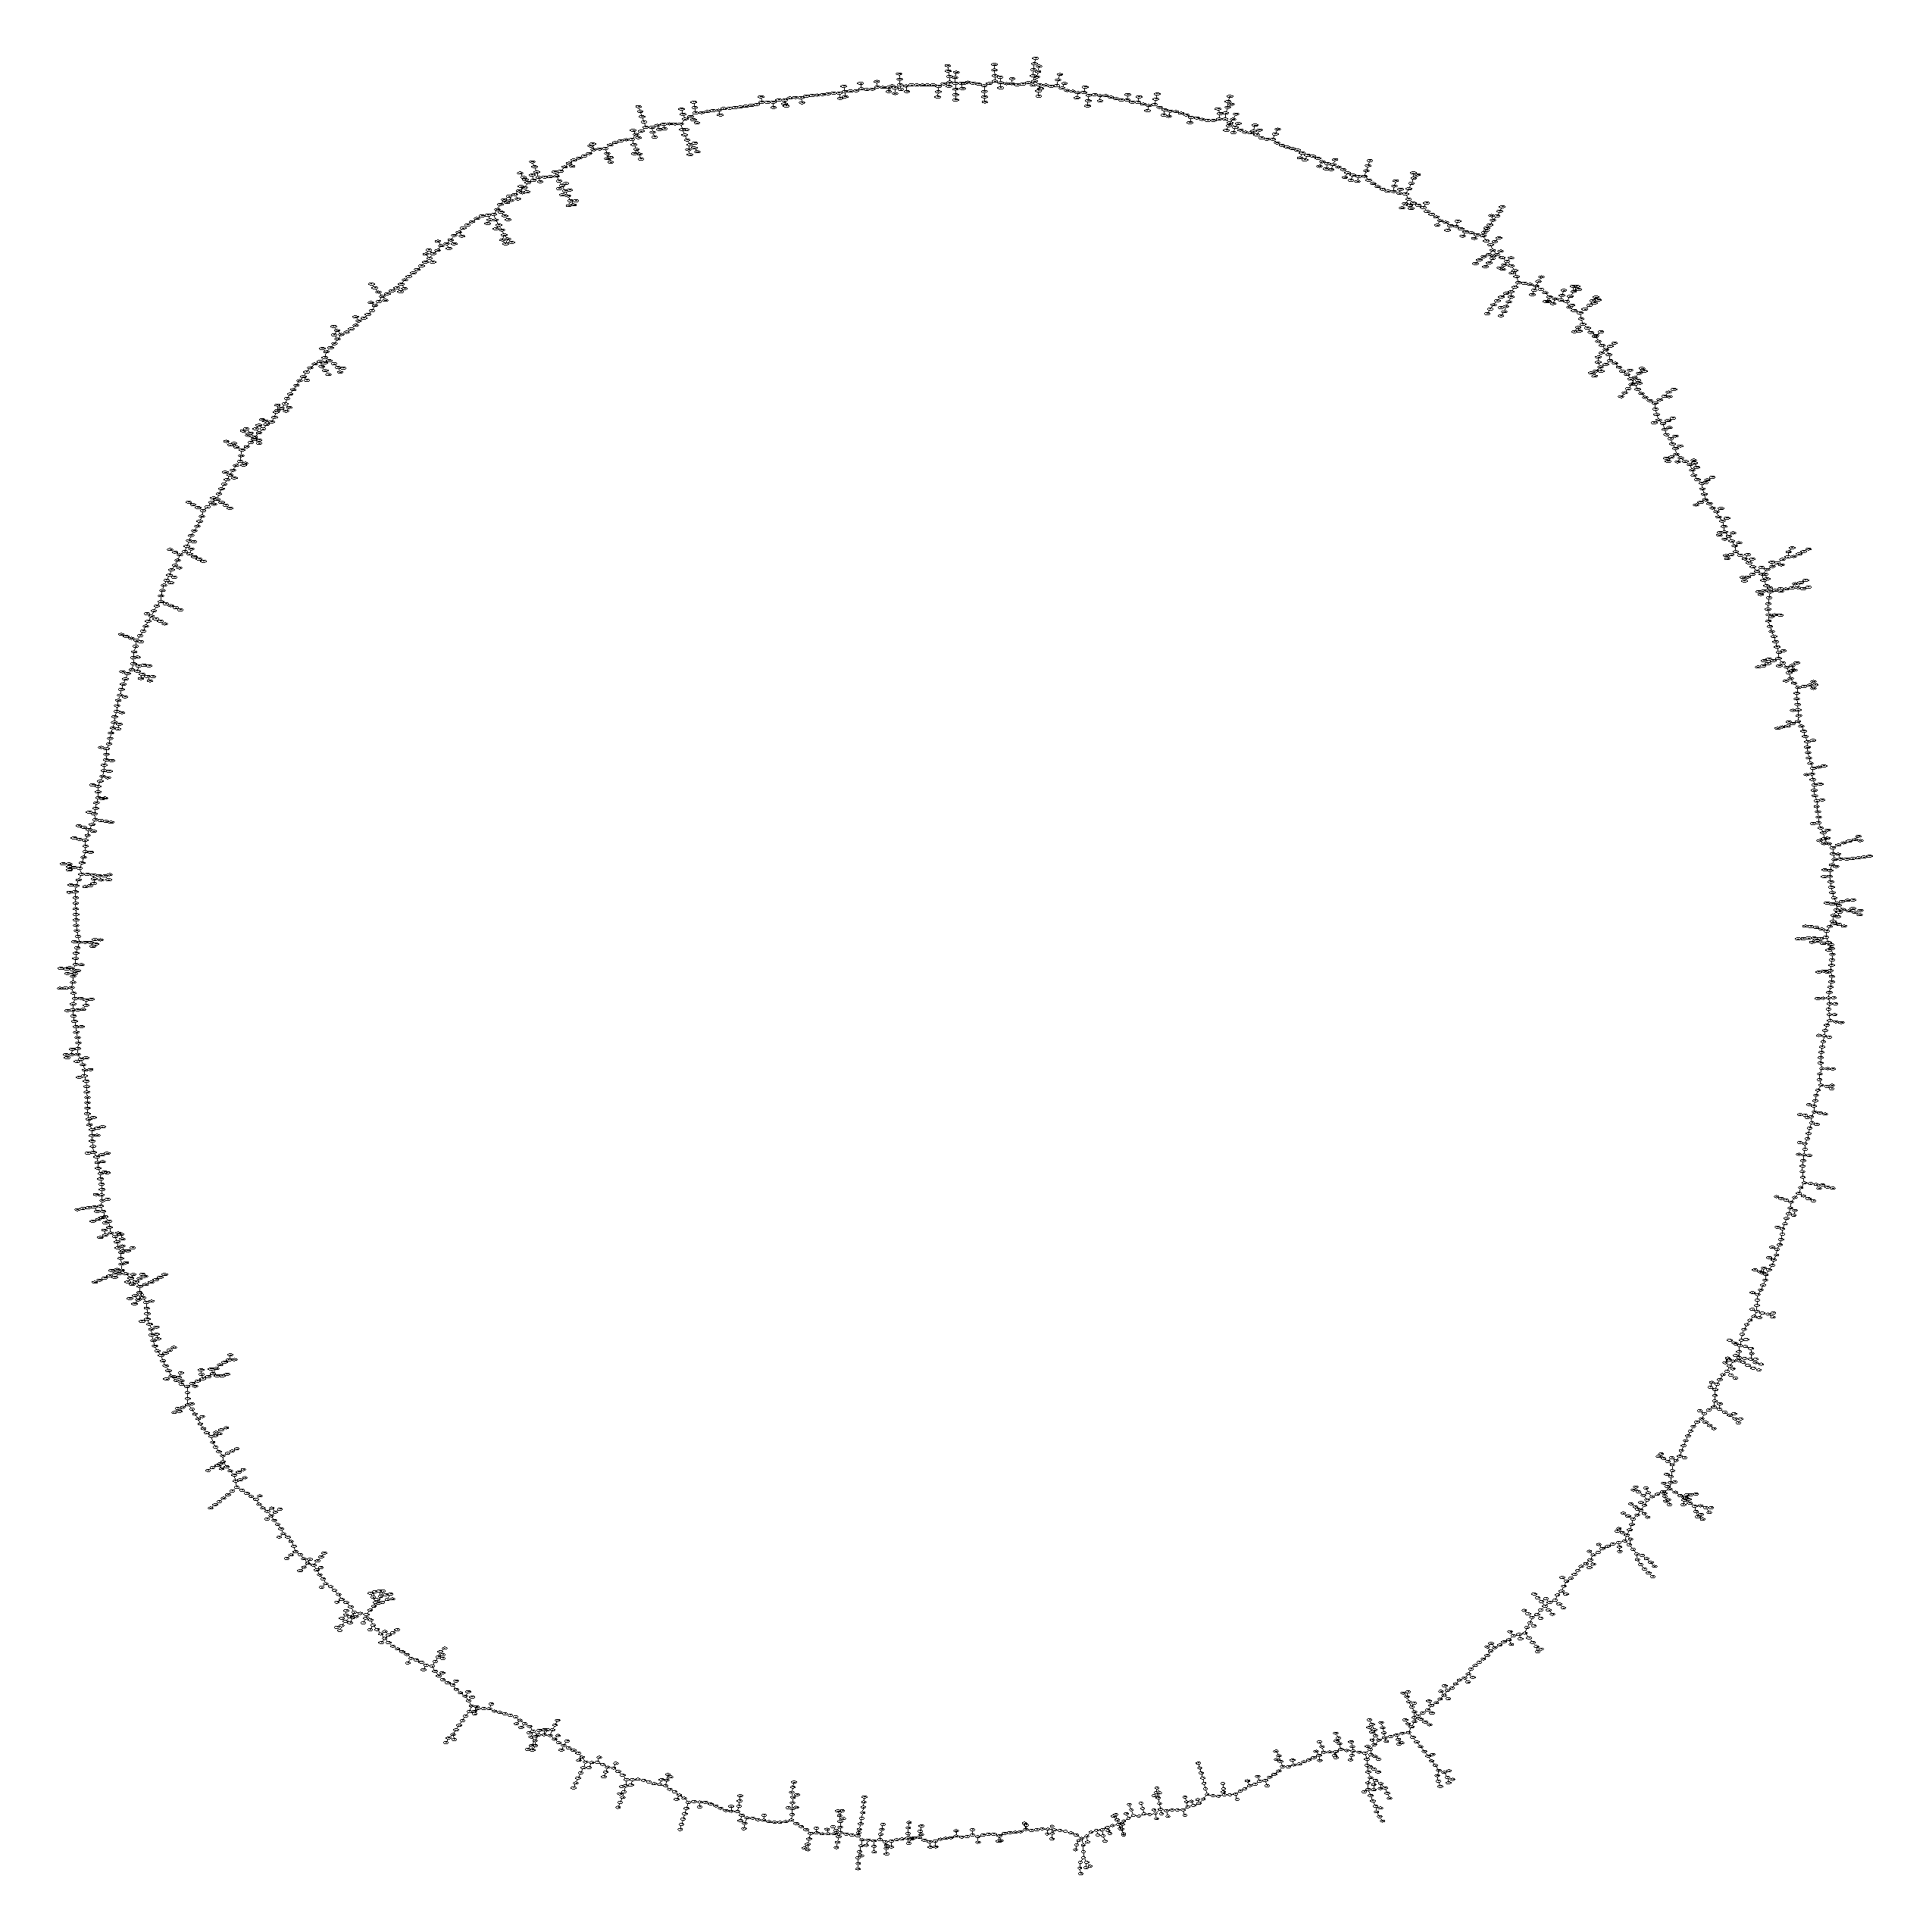
\includegraphics[width=3in]{figures/f3b010}
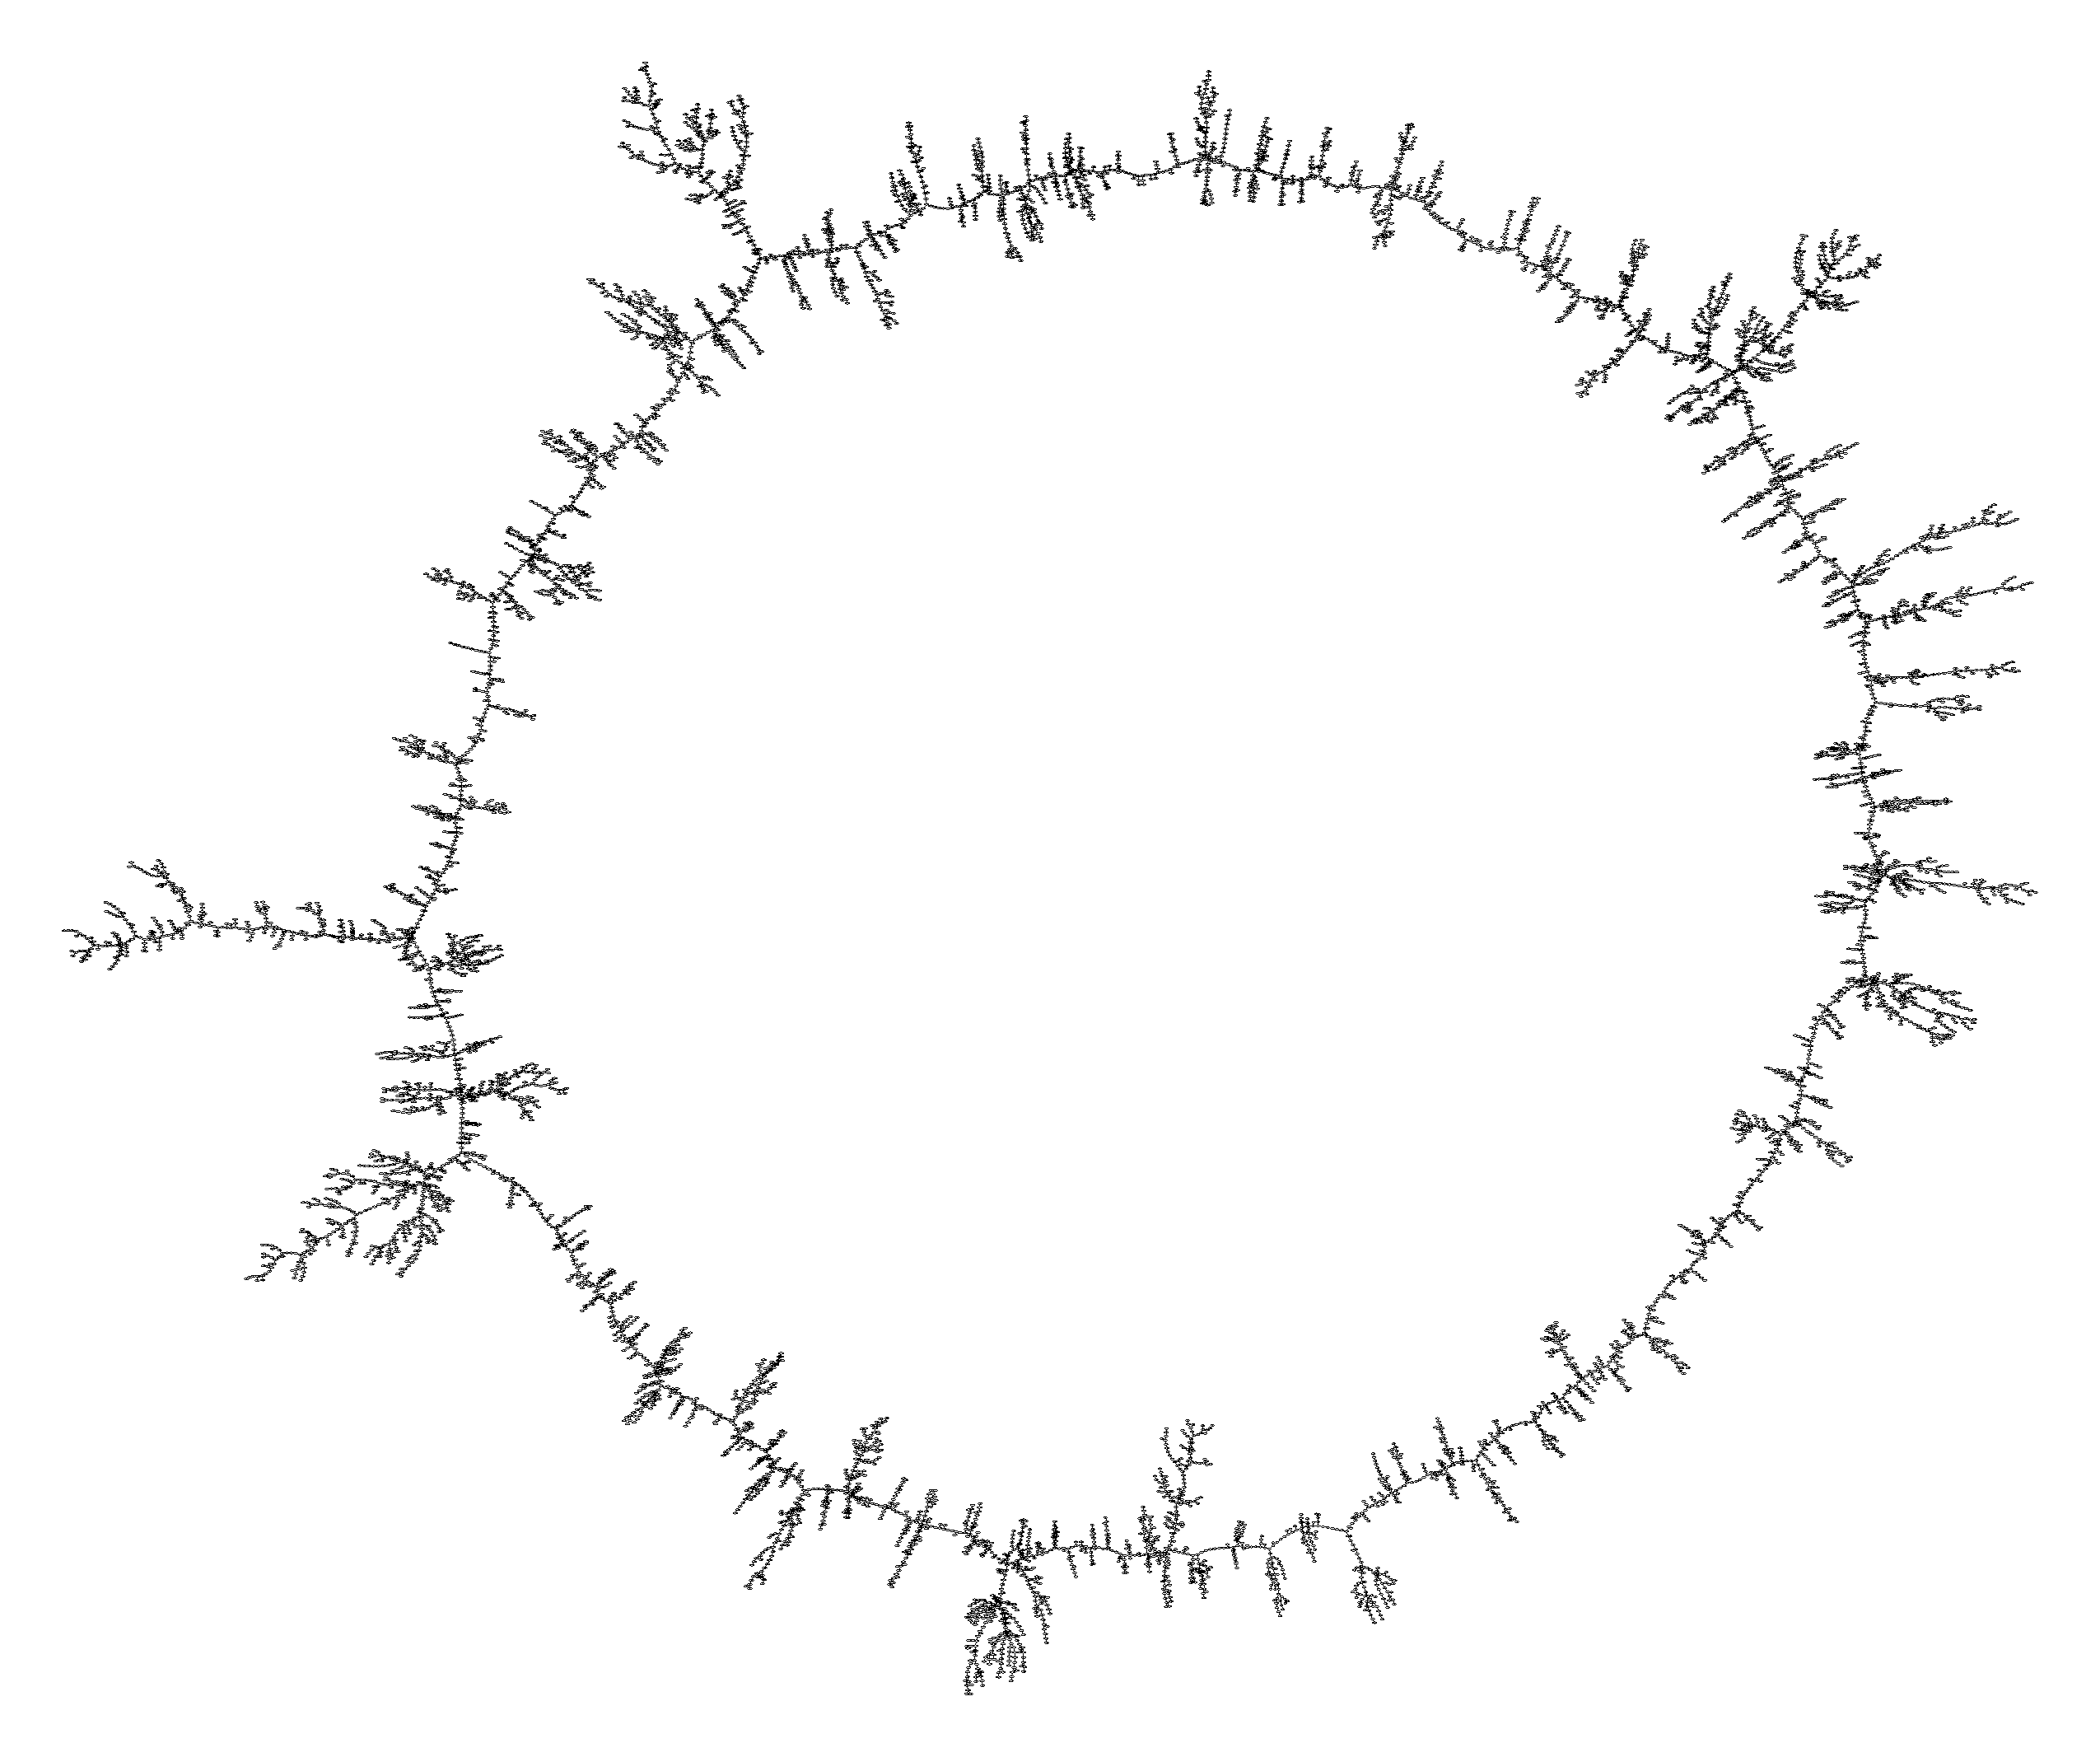
\includegraphics[width=3in]{figures/f3b015}
\caption{Graph visualizations demonstrating the decreasing 
fidelity of graph structure with increasing false positive rate. From 
top left to bottom right, the false positive rates are 0.01, 0.05, 0.10, 
and 0.15.}
\end{figure}

In addition, it is trivial to see that a linear increase in the false 
positive rate results in a linear increase in the number of expected 
neighbors for a particular k-mer. For an isolated k-mer (no adjacent 
``real'' k-mers), the calculation is 
E(erroneous neighbors)$ = 8 \times p_f$. This implies that the local graph 
structure breaks down in a linear fashion but offers no insight 
to how the global graph structure degrades.

\subsection{Percolation In K-mer Graphs}
As the false positive rate increases, there appears to be a sudden
transition between the point where graph traversal is possible and
when it is not. This rapid change resembles a phase transition in the
field of physics, which can be modelled using percolation theory. As
long as the false positive rate is below the percolation threshold (in
the subcritical phase), it is possible to traverse the graph. If the
false positive rate is at or above this (in the supercritical phase), then graph
traversal is infeasible. 

We explored the percolation threshold by randomly inserting 31-mers into Bloom
filters with increasing false positive rates and calculated the average
cluster size for each. Figure 2 demonstrates that the average cluster
size rapidly increases as the percolation threshold is approached,
which appears to be at a FP rate near 0.18 for k=31. This
graph also suggests that up to the percolation threshold, DNA assembly graph 
traversal is remains possible but becomes slower as the threshold is
approached.

\begin{figure}
\center{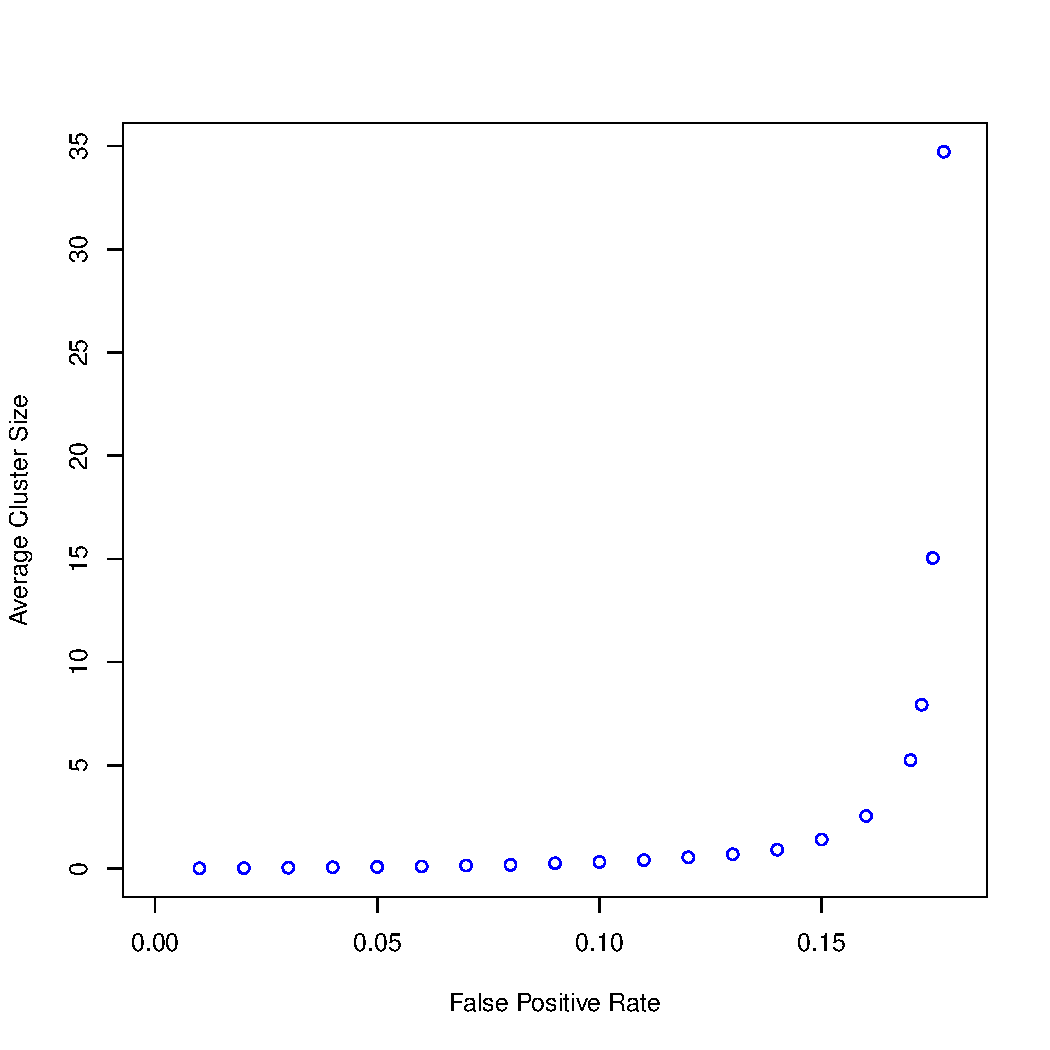
\includegraphics[width=5in]{k31}}
\caption{The average cluster size sharply increases as the false positive 
rate approaches the percolation threshold.
}
\end{figure}

Using the calculation method described in \emph{Methods} we found the 
percolation threshold for de Bruijn graphs to be $\sim0.183$. 
Furthermore, the percolation appears to be the same for 
different $k$, which suggests that the 
critical point is $k$ independent.
This implies that one can only add 18\% of the possible $4^k$ k-mers
before random data would percolate anyways. Using percolation theory to 
assess usability is limited in that it assumes
random k-mers to be added, while actual sequence data is a stream of
connected k-mers.

\subsection{Large-scale Graph Structure Retained to Percolation Threshold}
We demonstrate that the global connectivity of the graph is unlikely 
to change below the percolation threhold. We randomly generated 58bp long circular 
chromosomes and calculated the diameter at different false positive rates and averaged 
the results from multiple runs ($n=20$). The diameter 
of a connected component in a graph is defined as the length of the ``longest shortest'' 
path between any two vertices in the component. In our case, we only considered the 
paths where the start and end k-mer are not false positives. As Figure 3 shows, 
there is unlikely to 
be erroneous connections between pairs of ``real'' k-mers in the graph below the 
percolation threshold. Shortly after the percolation threshold, spurious connections 
between real k-mers are created, which lowers the diameter. For larger k, false connections 
between k-mers are even more unlikely since the shortest path between two k-mers 
with no overlap is $k$ in length.

\begin{figure}
\center{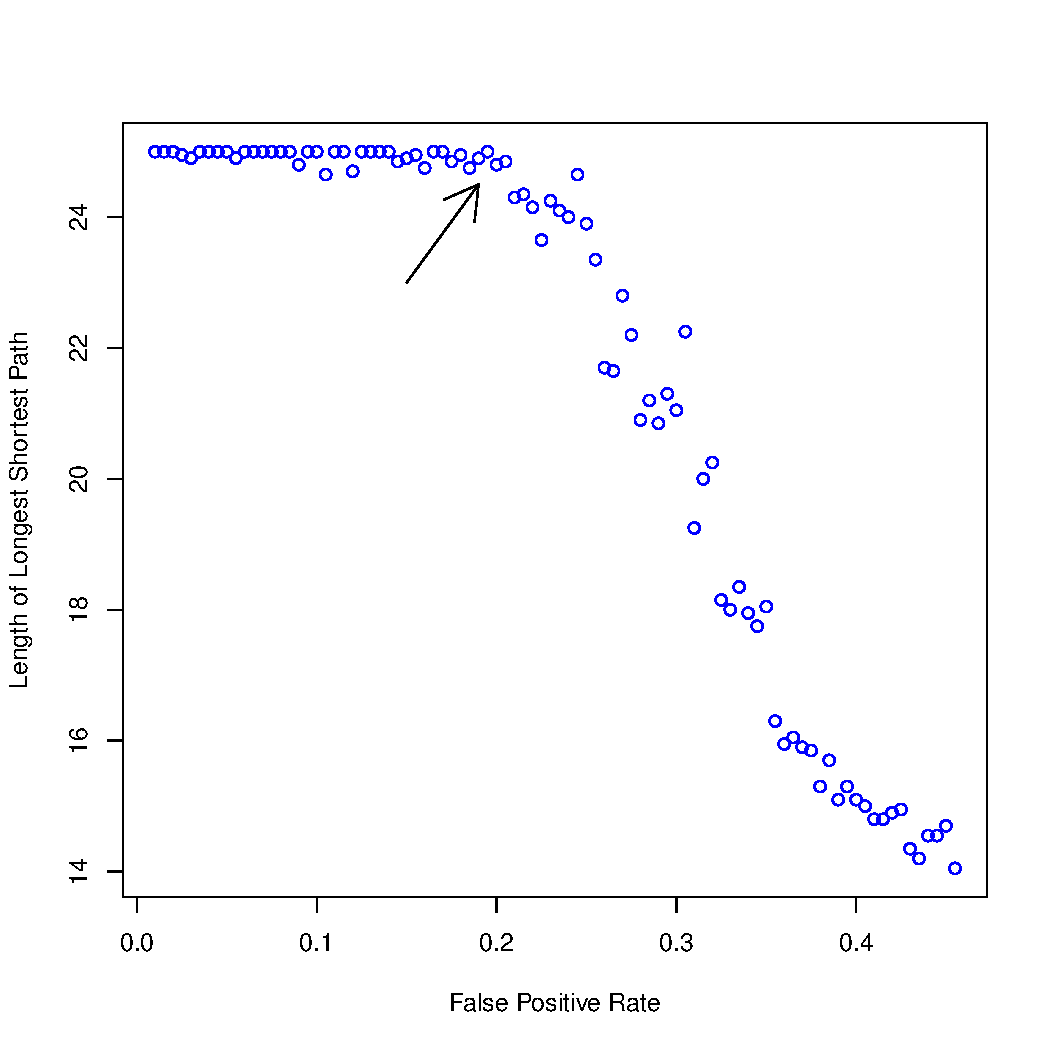
\includegraphics[width=5in]{figures/diameter}}
\caption{The length of the longest shortest path of randomly generated 58bp 
long circular chromosomes in 8-mer 
space for different false positive rates. Only real (non-error) k-mers are 
considered.}
\end{figure}

\subsection{Sequencing Errors Ecliple Errors From Graph Representation}
One important consideration when determining the usefulness of our k-mer
graph representation is how it compares to errors from massively
parallel sequencers such as Illumina. In de Bruijn graph-based
assemblers, sequencing errors add to the graph complexity and make it
more difficult to find high-quality paths for generating long,
accurate contigs. Since our approach generates
positive rate sequencing errors dominate the graph complexity
issue. We used an E. coli dataset provided by Illumina to compare
various graph invariants between the Illumina dataset, an exact
representation of the genome, and various inexact representations with
different false positive rates.

For these estimates, we used the genomic sequence from the E. coli strain 
MG1665 NC000913, which has a circular genome with $\sim 4.57e10^6$ bases. 
In theory, each of the k-mers that makes this
circular graph should have exactly one k-mer following it, but due to 
repeated and identical k-mers we found 716 interconnections in this graph 
already when using an exact representation. We repeated this procedure 
using a single hash table with $10^9$ bits of memory and found an excess of 
$67,608$ neighbors over the expected number, which corresponds to an error rate of 
$\sim 1.5\%$. For smaller memory 
sizes we found higher error rates (~14.0\% error for $10^8$ bits and 
~109\% for $10^7$ bits).

Nevertheless, when using 
the sequencing data from Illumina, if we use the $10^9$ bits of memory 
from before, we would fall above the percolation threshold which is 
about $2.39e10^9$ bits for the 
$4.17e10^8$ k-mers present in the Illumina dataset. 
If we use $10^{10}$ bits (10-fold more), the error rate is 
$\sim 133\%$. This clearly demonstrates that
the errors generated from sequencing dwarfs the error caused by false positives.

\section{Discussion}

\subsection{Bloom Filters Can Be Used To Accurately Store Large Assembly Graphs}
The compressible graph representation we have built on a Bloom filter
is an efficient way to store and traverse k-mer graphs.  Per k-mer
memory usage is low compared to approaches without false positives
and independent of k while k-mer node lookup and
local traversal are constant time.  The primary data structure can
also be implemented in constant memory.  This graph representation is
also extremely simple to implement and verify.

The probabilistic nature of the data structure is a significant
concern, but the collision rate and resulting increase in false local
connectivity are very predictable.  On a larger scale, we can link the
rate of increase in global connectivity from false positives to a
first-order phase transition, which lets us define a broad range of
parameters for which global graph structure is extremely accurate.
% @CTB Yes yes yes!
Within this range, the primary effect of decreasing memory is to increase
traversal computation.  Note that this also provides a systematic way
to trade time spent in traversal (computation) off against memory. As shown 
in Figure 2, the amount of traversal from each k-mer increases 
(affecting computation) as the false positive rate increases, which 
is determined by the amount of memory that is allocated to the data 
structure.

The effect of increasing false positive rate as ``error'' can be
compared to the effect of sequencing errors.  Sequencing error
introduces both false negatives (by eliminating ``true'' k-mers from
low coverage samples) and false positives.  False positives and
negatives from sequencing errors also often result in k-mers that are
a low Hamming distance from the true k-mer, which can result in
elaborate graph structures.  In contrast, the Bloom graph error is
entirely one-sided, only resulting in false positives; moreover, these
false positives are uncorrelated to the ``true'' k-mers from which
they arise, and generally contribute to local graph structure only 
in a linear fashion as the false positive rate increases.

Overall, the Bloom k-mer graph is an efficient data structure for
storing and traversing large k-mer graphs.

\subsection{Applying Bloom K-mer Graphs For DNA Sequence Assembly}
Bloom k-mer graphs will not be directly useful for traditional
approaches to DNA assembly, which rely on systematic heuristic
transformations of graph structure to find an optimal path through the
graph.  This is because the Bloom graph, as presented here, is limited
to representing k-mer graphs for a fixed k, and paths cannot readily
be compacted or eliminated.
% @CTB What did I mean ``for a fixed k''?  I don't know of any DBG
% reps that don't use a fixed k!

There are many uses, however, for an extremely scalable
constant-memory graph representation.  Below we discuss the use of the
Bloom k-mer graph data structure as a lens for exploring graph
properties and filtering data sets.

For low-coverage samples, assembly graphs may contain many small
unconnected components, that represent unconnected sequences.
% @CTB why?  Beacuse of low coverage! Reiterate I guess.
Sequences contributing to these unconnected components can be safely
eliminated from the originating data sets without affecting the final
assembly.  This can be done efficiently with a simple limited depth
graph search algorithm. Since connected components in the graph 
are unlikely to erroneously connect when the false positive rate 
is below the percolation threshold, graph traversal is only affected 
by the minor changes to the local graph structure.

More generally, assembly graphs may contain many disconnected
subgraphs, due to the structure of the source data (e.g. transcriptome
or population sequencing) or because of low coverage.  These subgraphs
can safely be partitioned into different graphs without affecting the
final assembly, reducing the memory and computation required for
assembly of the whole to that required for the largest subgraph.
% @CTB discuss local vs global structure changes from FP on this.

The Bloom k-mer graph can also be used to do de novo repeat discovery
in collections of unassembled reads.  This in turn can be applied to
filtering of repeats prior to assembly (ref Hydra), or for isolating
repeats from shallow or exploratory sequencing efforts.
% @JAP I can't find the Hydra citation

It should also be possible to adapt sequence structure (e.g. ORF),
homology (BLAST), and domain search (HMMER) algorithms to search this
graph structure instead of searching either unassembled reads or
assemblies.  Because assembly graphs implicitly collapse identical
sequences into a single path, this may be a more scalable approach to
targetted-gene analysis for metagenomics than current approaches
(which rely on searching individual reads).  Also note that, unlike
sequencing errors, the false positives in the Bloom graph will
generally bear no resemblance to biologically valid matches.

The Bloom k-mer graph could also be used to develop connectivity-based
read trimming and correction algorithms.  For example, low-abundance
reads that contribute to ``spurs'' or ``sidings'' in otherwise
high-coverage regions could be corrected to match the
consensus, or trimmed to eliminate the divergent sequence.

One particularly intriguing option is to use the memory-efficient and
scalable Bloom k-mer graph representation as a component of a hybrid
assembler.  The k-mer graph approach could be used to identify
reads that belong to high-complexity regions, and extract them for
later resolution with more targetted approaches, e.g. an OLC assembler.

\subsection{Dramatic Scaling}
It is clear that sequencing capacity will continue to outpace Moore's 
law and new methods must address this. Our graph representation allows 
for excellent scaling capabilities at the cost of a manageable false positive rate. 
As mentioned previously, $\sim 6.22$ bits per k-mer are required for a 
false positve rate of 5\%, which implies that modern supercomputers with 
over 512GB of memory can handle graphs with hundreds of billions of k-mers.

Another consideration is that assembly is generally difficult to parallelize. 
ABySS and Contrail (citation?), for example, place different parts of the 
graph on separate nodes. However, this can hinder performance due to 
network latency. Having the ability to hold the entire graph in memory 
before spreading the graph to different nodes can guarantee that nodes 
will not need to query one another frequently, if at all. A smaller memory 
footprint can also mean that the entire assembly could be performed on 
a single node, if computational resources are limited.

Finally, though so-called ``third-generation'' sequencers are showing promise with 
longer reads and better error rates, we argue that improvements in these 
areas will not solve the scaling issue in certain domains. In particular, 
mRNAseq and metagenomics datasets are still lacking in coverage to be 
fully useful in many cases. Differential expression detection and/or assembly 
of low-expressed genes are difficult without very deep coverage. This implies 
that the required coverage level for an mRNAseq dataset will not change, 
and thus the size of the dataset. Furthermore, many environmental samples with 
diverse microbial communities are estimated to require several terabases of sequencing 
in order to achieve a modest coverage level (citation?). In both of these domains, better 
scaling algorithms are needed to handle these complex assemblies. 

\subsection{Concluding Remarks}
We have shown that representing a k-mer graph on a Bloom filter-like data 
structure can create an inexact, yet lightweight graph representation of 
a k-mer graph. This inexactness can be precisely known based on the occupancy 
of each hash table, and we demonstrated that our approach is still useful 
below a specific false positive rate. We conclude that while this representation 
may not be ideal for a final assembly, it can be very useful for pre-filtering 
strategies and solving the scaling and memory bottleneck problems that we 
currently face in sequence assembly.

\subsection{Acknowledgements}

Jim Cole and Jordan Fish.  Qingpeng.  Adina.

\bibliographystyle{abbrv}
\bibliography{kmer-percolation}
\end{document}


